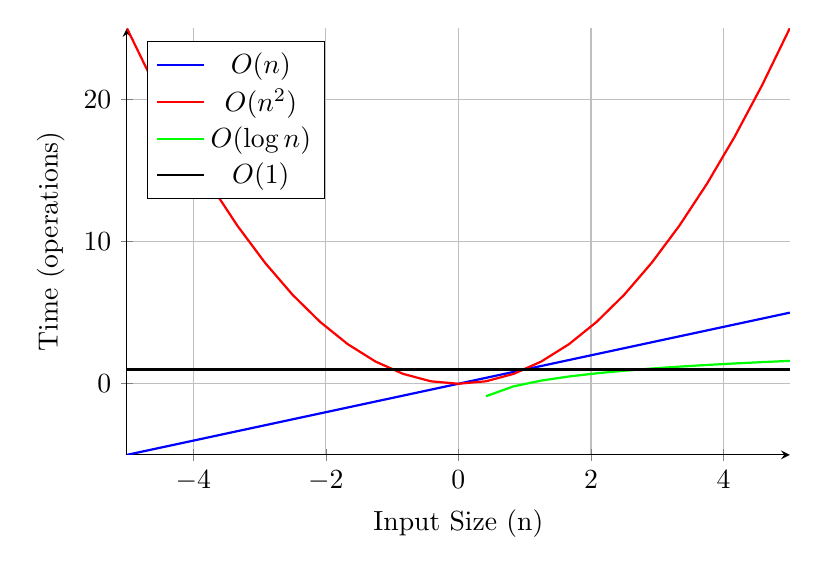
\begin{tikzpicture}
    \begin{axis}[
        xlabel={Input Size (n)},
        ylabel={Time (operations)},
        legend pos=north west,
        grid=major,
        axis lines=left,
        width=10cm,
        height=7cm
    ]
    % O(n)
    \addplot[blue, thick] {x};
    \addlegendentry{$O(n)$}

    % O(n^2)
    \addplot[red, thick] {x^2};
    \addlegendentry{$O(n^2)$}

    % O(log n)
    \addplot[green, thick] {ln(x)};
    \addlegendentry{$O(\log n)$}

    % O(1)
    \addplot[black, thick] {1};
    \addlegendentry{$O(1)$}
    \end{axis}
\end{tikzpicture}
